\section{Design}
\subsection{Design Overview}

\begin{figure}[tbh]
\centering
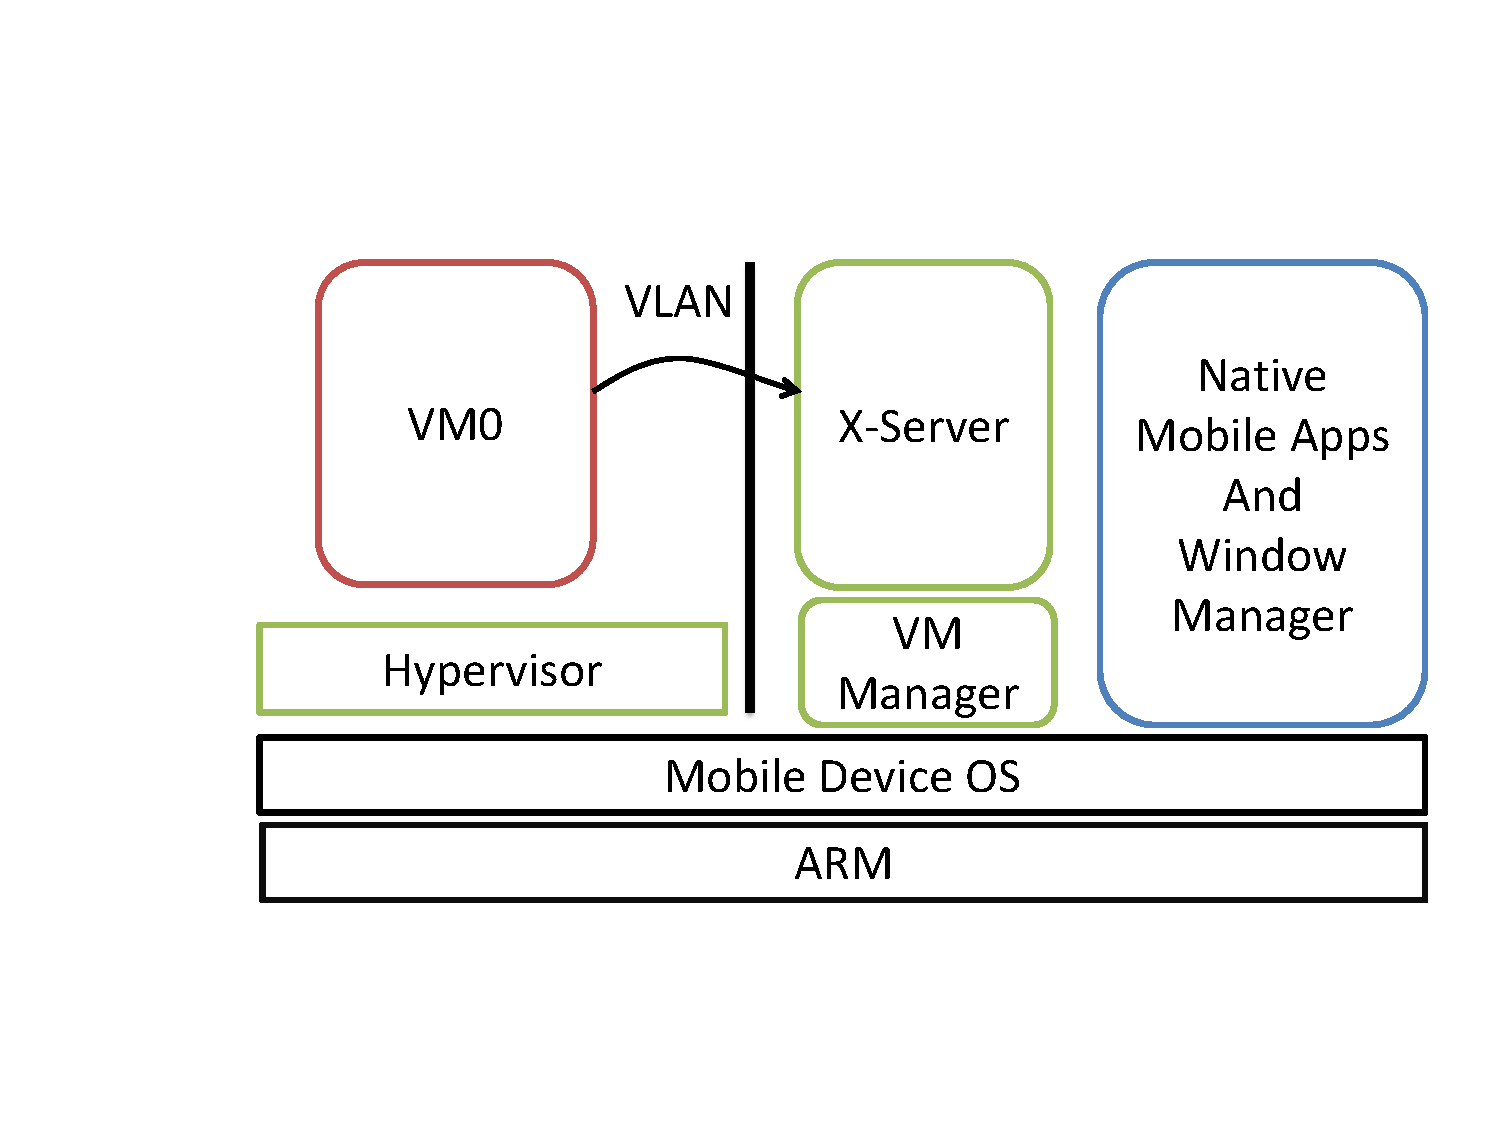
\includegraphics[width=1.0\columnwidth]{arch}
\caption{Architecture diagram}
\label{fig:arch}
\end{figure}

\label{sec:proposedarch}
Our architecture has two main components: the virtualization framework, and the integration front-end.  The virtualization framework contains the hypervisor (KVM, UserMode Linux, or L4 based) or container-ready kernel (Linux Containers-LXC) as well as each of the spawned VMs or containers (see Figure \ref{fig:arch}).  A VM would contain a thin OS for running the third-party application.  A container would contain one or more application.  Initially we intended to explore both x86-based Operating Systems as well as ARM based systems.  However, initial results show that x86-based Operating Systems will be far too slow.  Although an x86-based OS would have enabled a more diverse set of target applications, ARM-based systems have less virtualization overhead and some options may not be prohibitively slow. %Each of the VMs will headless themselves, but will render their applications by connecting to the native X-server. *Is this still true?* \\

The other component is the integration front-end.  This contains a light X-server that has been integrated into the host OS, and also contains the VM/container manager.  The manager will either run inside the X-server as a native application (ARM-based), or as a separate application within the host OS or containers.  The manager will be the user interface that controls launching, switching, suspending, resuming, migrating the VMs or containers, as well as ensuring the X-server is running properly. %Most of this actual logic and functionality will be implemented by the hypervisor in the virtualization framework. \\

A shared X-server removes rendering overhead from each VM or container and reduces the complexity in composing the UI. We choose to share the rendering state between third-party applications for performance reasons and simplicity of design, but ensure isolation from native applications.  Additionally the X-server will be running native code, which will allow for it to be less CPU intensive than running inside a VM or container. \\

We aim to make the virtualization framework device independent, which is important because we anticipate this to be the more complex component.  The integration front-end will have to be ported for each new device we support, but we will strive to make its implementation simple. Our first implementation will focus on one particular device and OS and support live migration of applications from desktops. \\

In summary, we propose to leverage an existing virtualization environment to build a secure, usable and portable framework for mobile device virtualization. Our contributions will be focused on providing the ability for live migration of applications with deep integration to the mobile device. Our proposed security model is an effective method to isolate applications and we find that our design ideas are similar to other recent efforts \cite{grier2008secure} in isolating untrusted code.

\subsection{QEMU + X server}
\subsection{Other Virtualization Techniques}
\subsubsection{KVM}
\subsubsection{User Mode Linux}
\subsubsection{Linux Containers}
Linux Containers (LXC) implement OS-level virtualization in order to run a number of isolated virtual environments on a single host.  LXC differs from conventional virtualization technices, which generally require the installation of guest OSes.  Unlike with conventional virtualization, LXC has almost no overhead as it does not require guest OSes or dynamic translation.  On the other hand, because it is a OS-level virtualization technique and runs processes on a Linux kernel, other OSes such as Windows and other UNIXes (BSD or OSX) can not be used as containers.  

The main obstacle to using Linux Containers are the requirements.  LXC requires a Linux kernel version 2.6.27 or greater, and the Pre is running 2.6.24.  The kernel functionality would have to be back ported in order to work with the Pre.  The Android is running 2.6.29; however, porting the LXC tools to Android will likely be very difficult.
